% Options for packages loaded elsewhere
\PassOptionsToPackage{unicode}{hyperref}
\PassOptionsToPackage{hyphens}{url}
%
\documentclass[
]{article}
\usepackage{lmodern}
\usepackage{amssymb,amsmath}
\usepackage{ifxetex,ifluatex}
\ifnum 0\ifxetex 1\fi\ifluatex 1\fi=0 % if pdftex
  \usepackage[T1]{fontenc}
  \usepackage[utf8]{inputenc}
  \usepackage{textcomp} % provide euro and other symbols
\else % if luatex or xetex
  \usepackage{unicode-math}
  \defaultfontfeatures{Scale=MatchLowercase}
  \defaultfontfeatures[\rmfamily]{Ligatures=TeX,Scale=1}
\fi
% Use upquote if available, for straight quotes in verbatim environments
\IfFileExists{upquote.sty}{\usepackage{upquote}}{}
\IfFileExists{microtype.sty}{% use microtype if available
  \usepackage[]{microtype}
  \UseMicrotypeSet[protrusion]{basicmath} % disable protrusion for tt fonts
}{}
\makeatletter
\@ifundefined{KOMAClassName}{% if non-KOMA class
  \IfFileExists{parskip.sty}{%
    \usepackage{parskip}
  }{% else
    \setlength{\parindent}{0pt}
    \setlength{\parskip}{6pt plus 2pt minus 1pt}}
}{% if KOMA class
  \KOMAoptions{parskip=half}}
\makeatother
\usepackage{xcolor}
\IfFileExists{xurl.sty}{\usepackage{xurl}}{} % add URL line breaks if available
\IfFileExists{bookmark.sty}{\usepackage{bookmark}}{\usepackage{hyperref}}
\hypersetup{
  hidelinks,
  pdfcreator={LaTeX via pandoc}}
\urlstyle{same} % disable monospaced font for URLs
\usepackage[margin=1in]{geometry}
\usepackage{color}
\usepackage{fancyvrb}
\newcommand{\VerbBar}{|}
\newcommand{\VERB}{\Verb[commandchars=\\\{\}]}
\DefineVerbatimEnvironment{Highlighting}{Verbatim}{commandchars=\\\{\}}
% Add ',fontsize=\small' for more characters per line
\usepackage{framed}
\definecolor{shadecolor}{RGB}{248,248,248}
\newenvironment{Shaded}{\begin{snugshade}}{\end{snugshade}}
\newcommand{\AlertTok}[1]{\textcolor[rgb]{0.94,0.16,0.16}{#1}}
\newcommand{\AnnotationTok}[1]{\textcolor[rgb]{0.56,0.35,0.01}{\textbf{\textit{#1}}}}
\newcommand{\AttributeTok}[1]{\textcolor[rgb]{0.77,0.63,0.00}{#1}}
\newcommand{\BaseNTok}[1]{\textcolor[rgb]{0.00,0.00,0.81}{#1}}
\newcommand{\BuiltInTok}[1]{#1}
\newcommand{\CharTok}[1]{\textcolor[rgb]{0.31,0.60,0.02}{#1}}
\newcommand{\CommentTok}[1]{\textcolor[rgb]{0.56,0.35,0.01}{\textit{#1}}}
\newcommand{\CommentVarTok}[1]{\textcolor[rgb]{0.56,0.35,0.01}{\textbf{\textit{#1}}}}
\newcommand{\ConstantTok}[1]{\textcolor[rgb]{0.00,0.00,0.00}{#1}}
\newcommand{\ControlFlowTok}[1]{\textcolor[rgb]{0.13,0.29,0.53}{\textbf{#1}}}
\newcommand{\DataTypeTok}[1]{\textcolor[rgb]{0.13,0.29,0.53}{#1}}
\newcommand{\DecValTok}[1]{\textcolor[rgb]{0.00,0.00,0.81}{#1}}
\newcommand{\DocumentationTok}[1]{\textcolor[rgb]{0.56,0.35,0.01}{\textbf{\textit{#1}}}}
\newcommand{\ErrorTok}[1]{\textcolor[rgb]{0.64,0.00,0.00}{\textbf{#1}}}
\newcommand{\ExtensionTok}[1]{#1}
\newcommand{\FloatTok}[1]{\textcolor[rgb]{0.00,0.00,0.81}{#1}}
\newcommand{\FunctionTok}[1]{\textcolor[rgb]{0.00,0.00,0.00}{#1}}
\newcommand{\ImportTok}[1]{#1}
\newcommand{\InformationTok}[1]{\textcolor[rgb]{0.56,0.35,0.01}{\textbf{\textit{#1}}}}
\newcommand{\KeywordTok}[1]{\textcolor[rgb]{0.13,0.29,0.53}{\textbf{#1}}}
\newcommand{\NormalTok}[1]{#1}
\newcommand{\OperatorTok}[1]{\textcolor[rgb]{0.81,0.36,0.00}{\textbf{#1}}}
\newcommand{\OtherTok}[1]{\textcolor[rgb]{0.56,0.35,0.01}{#1}}
\newcommand{\PreprocessorTok}[1]{\textcolor[rgb]{0.56,0.35,0.01}{\textit{#1}}}
\newcommand{\RegionMarkerTok}[1]{#1}
\newcommand{\SpecialCharTok}[1]{\textcolor[rgb]{0.00,0.00,0.00}{#1}}
\newcommand{\SpecialStringTok}[1]{\textcolor[rgb]{0.31,0.60,0.02}{#1}}
\newcommand{\StringTok}[1]{\textcolor[rgb]{0.31,0.60,0.02}{#1}}
\newcommand{\VariableTok}[1]{\textcolor[rgb]{0.00,0.00,0.00}{#1}}
\newcommand{\VerbatimStringTok}[1]{\textcolor[rgb]{0.31,0.60,0.02}{#1}}
\newcommand{\WarningTok}[1]{\textcolor[rgb]{0.56,0.35,0.01}{\textbf{\textit{#1}}}}
\usepackage{graphicx,grffile}
\makeatletter
\def\maxwidth{\ifdim\Gin@nat@width>\linewidth\linewidth\else\Gin@nat@width\fi}
\def\maxheight{\ifdim\Gin@nat@height>\textheight\textheight\else\Gin@nat@height\fi}
\makeatother
% Scale images if necessary, so that they will not overflow the page
% margins by default, and it is still possible to overwrite the defaults
% using explicit options in \includegraphics[width, height, ...]{}
\setkeys{Gin}{width=\maxwidth,height=\maxheight,keepaspectratio}
% Set default figure placement to htbp
\makeatletter
\def\fps@figure{htbp}
\makeatother
\setlength{\emergencystretch}{3em} % prevent overfull lines
\providecommand{\tightlist}{%
  \setlength{\itemsep}{0pt}\setlength{\parskip}{0pt}}
\setcounter{secnumdepth}{-\maxdimen} % remove section numbering

\author{}
\date{\vspace{-2.5em}}

\begin{document}

\hypertarget{lanpanalysis}{%
\section{lanpAnalysis}\label{lanpanalysis}}

lanpAnalysis: (Lung Adenocarcinoma Neoantigen Patient Analysis) is an R
package that aims to analyze patient peptide data, for probable
HLA-I-binding neoantigens that may be significant for lung
adenocarcinoma immunotherapy. In recent years, neoantigens have been be
an immunotherapy target, as they may produce the rejection of tumours.
lanpAnalysis streamlines this process by indexing and analyzing a
patient's genes, and returns cruicial information on the presence of
these neoantigens, their relative affinities to HLA Alleles, and their
location within the gene.

\hypertarget{installation}{%
\subsection{Installation}\label{installation}}

You can install the released version of lanpAnalysis from
\href{https://github.com/}{GitHub} with:

\begin{Shaded}
\begin{Highlighting}[]
\KeywordTok{require}\NormalTok{(}\StringTok{"devtools"}\NormalTok{)}
\NormalTok{devtools}\OperatorTok{::}\KeywordTok{install_github}\NormalTok{(}\StringTok{"<GitHubUserName>/<PackageName>"}\NormalTok{, }\DataTypeTok{build_vignettes =} \OtherTok{TRUE}\NormalTok{)}
\KeywordTok{library}\NormalTok{(}\StringTok{"<PackageName>"}\NormalTok{)}
\end{Highlighting}
\end{Shaded}

\hypertarget{overview}{%
\subsection{Overview}\label{overview}}

ls(``package:'')

The full information related to the functions in lanpAnalysis are
provided in the function's man pages, all of which are open when typing
lanpAnalysis::\ldots{} The ultimate aim of the package is to provide a
graphical output to the patient's neoantigens that were discovered in
their genes. There are 2 main outputs, one that appears as a graphical
output noting the discovered neoantigens, their positions in the gene,
and the binding affinity between the neoantigen and the HLA allele,
which can be coloured according to the confidence level between the
mutation and the HLA allele. An example is directly below:

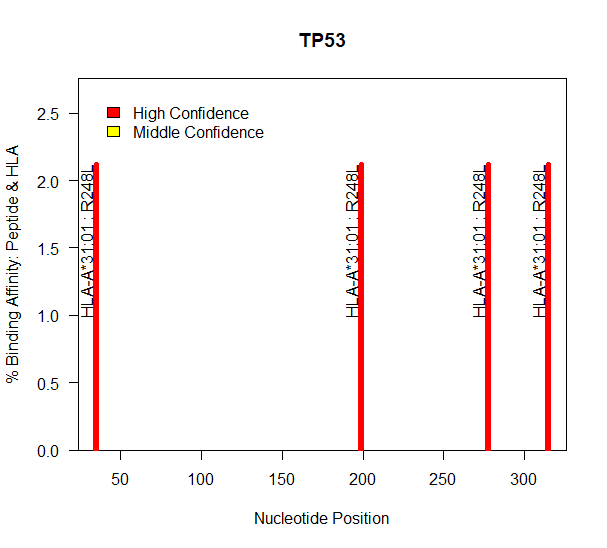
\includegraphics{./inst/extdata/location_plot.png}

This is the code to make this graphical output, with all files included
in the package:

\begin{Shaded}
\begin{Highlighting}[]
\KeywordTok{plot_mutation_location}\NormalTok{(}\StringTok{"TP53"}\NormalTok{, tp53mutated3times, }\DataTypeTok{confidence =} \DecValTok{1}\NormalTok{)}
\end{Highlighting}
\end{Shaded}

The other graphical output ranks the binding affinities of neoantigens,
and produces a barplot with this data. It can be coloured depending on
confidence levels or binding levels (You can read more about this in the
below function's man page) An example is directly below:

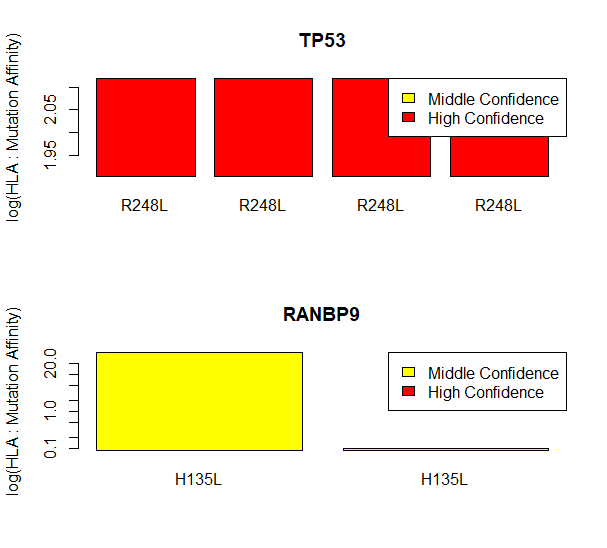
\includegraphics{./inst/extdata/plotWithConfidence.png}

This is the code to make this graphical output, with all files included
in the package:

\begin{Shaded}
\begin{Highlighting}[]
\NormalTok{lanpAnalysis}\OperatorTok{::}\KeywordTok{patient_affinity_visualizer}\NormalTok{(testingGeneSet, }\DataTypeTok{colNum=}\DecValTok{1}\NormalTok{, }\DataTypeTok{colorFlag=}\DecValTok{2}\NormalTok{)}
\end{Highlighting}
\end{Shaded}

\hypertarget{contributions}{%
\subsection{Contributions}\label{contributions}}

This package was built with R base packages: graphics, and stats; it is
suggested that you download testthat as well. It uses stringr as well,
which you can read on below in the references {[}3{]}. The database that
was utilized for this package `lungData' has been modified from database
dbPepNeo {[}1{]}

\hypertarget{references}{%
\section{References}\label{references}}

{[}1{]} Xiaoxiu Tan, Daixi Li, Pengjie Huang, Xingxing Jian, Huihui Wan,
Guangzhi Wang, Yuyu Li, Jian Ouyang, Yong Lin, Lu Xie, dbPepNeo: a
manually curated database for human tumor neoantigen peptides, Database,
Volume 2020, 2020, baaa004,
\url{https://doi.org/10.1093/database/baaa004}

{[}2{]} (Context information about Neoantigen was found here. I did not
derive an idea from this article, but I learned about neoantigens here,
and if you need information, this is the place to start) Evolution of
Neoantigen Landscape during Immune Checkpoint Blockade in Non--Small
Cell Lung Cancer Valsamo Anagnostou, Kellie N. Smith, Patrick M. Forde,
Noushin Niknafs, Rohit Bhattacharya, James White, Theresa Zhang, Vilmos
Adleff, Jillian Phallen, Neha Wali, Carolyn Hruban, Violeta B. Guthrie,
Kristen Rodgers, Jarushka Naidoo, Hyunseok Kang, William Sharfman,
Christos Georgiades, Franco Verde, Peter Illei, Qing Kay Li, Edward
Gabrielson, Malcolm V. Brock, Cynthia A. Zahnow, Stephen B. Baylin,
Robert B. Scharpf, Julie R. Brahmer, Rachel Karchin, Drew M. Pardoll and
Victor E. Velculescu DOI: 10.1158/2159-8290.CD-16-0828 Published March
2017 {[}3{]}
\url{https://cran.r-project.org/web/packages/stringr/vignettes/stringr.html}

\hypertarget{acknowledgements}{%
\section{Acknowledgements}\label{acknowledgements}}

This package was developed as part of an assessment for 2020 BCB410H:
Applied Bioinformatics, University of Toronto, Toronto, CANADA.

\end{document}
